% kapitel2.tex
\chapter{Implemented Changes}
\label{chapter:implementedChanges}

This work extends Tour4Me, which is an application written in C++ and HTML. 
The implemented interface uses C\# as its programming language to enable easy porting of the webapplication to a desktop or mobile application.
To improve the query times, a spatial database was added. 
Reasons for and positive effects of this decision are described in the following section.

Furthermore, not only the language and data access was changed.
New options and parameters to improve the customizability of preferences for a generated tour were added as well.
These changes had to be incorporated into an upgraded frontend design (see sections \ref{subsec:interfaceAndFrontendChanges} and \ref{sec:parameterChanges}) as well as into the backend and all solvers (see section \ref{sec:algorithmicChanges}). 


\section{Application}
\label{sec:application}

\subsection{New Architecture}
\label{sec:newArchitecture}

\begin{figure}[H]
	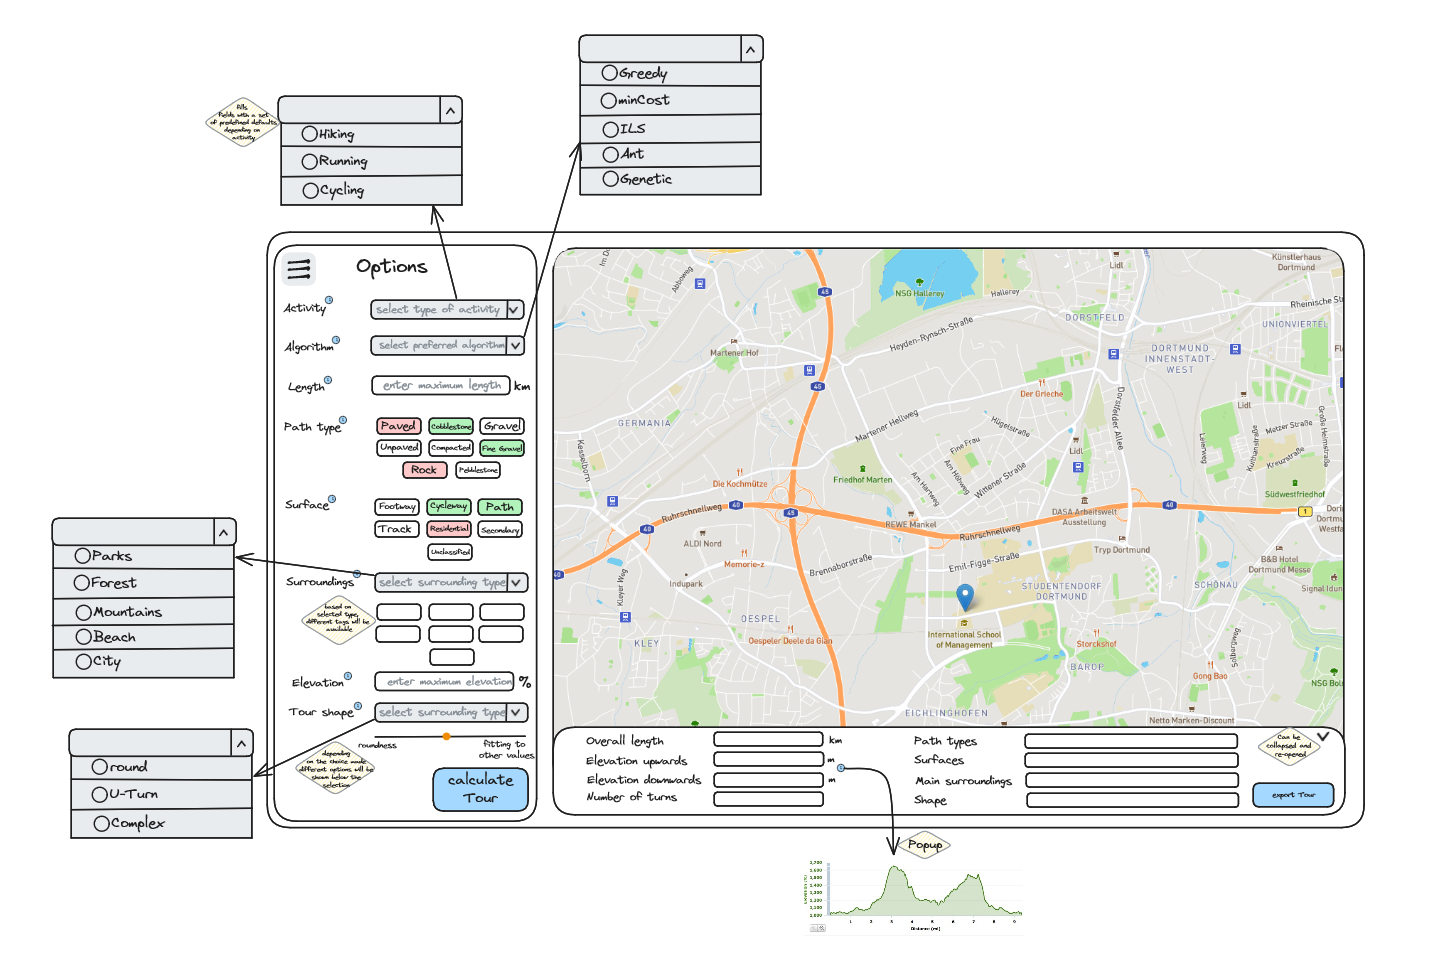
\includegraphics[width=0.9\linewidth]{bilder/Concept new Frontend design.png}
	\caption{Design concept for the frrontend view, including descriptions for drop-downs and pop-ups}
	\label{fig:frontendConcept}
\end{figure}

\subsection{Database}
\label{subsection:database}

\subsection{Interface and Frontend changes}
\label{subsec:interfaceAndFrontendChanges}

\section{Algorithmic changes}
\label{sec:algorithmicChanges}

\subsection{Ant Colony}
\label{subsec:antColonyImplementation}

\subsection{Genetic Algorithms}
\label{subsec:geneticAlgorithmsImplementation}

\subsection{Simulated Annealing}
\label{subsec:simulatedAnnealingImplementation}

\section{Parameter changes}
\label{sec:parameterChanges}

